\begin{comment}
\begin{figure}[t]
\begin{center}
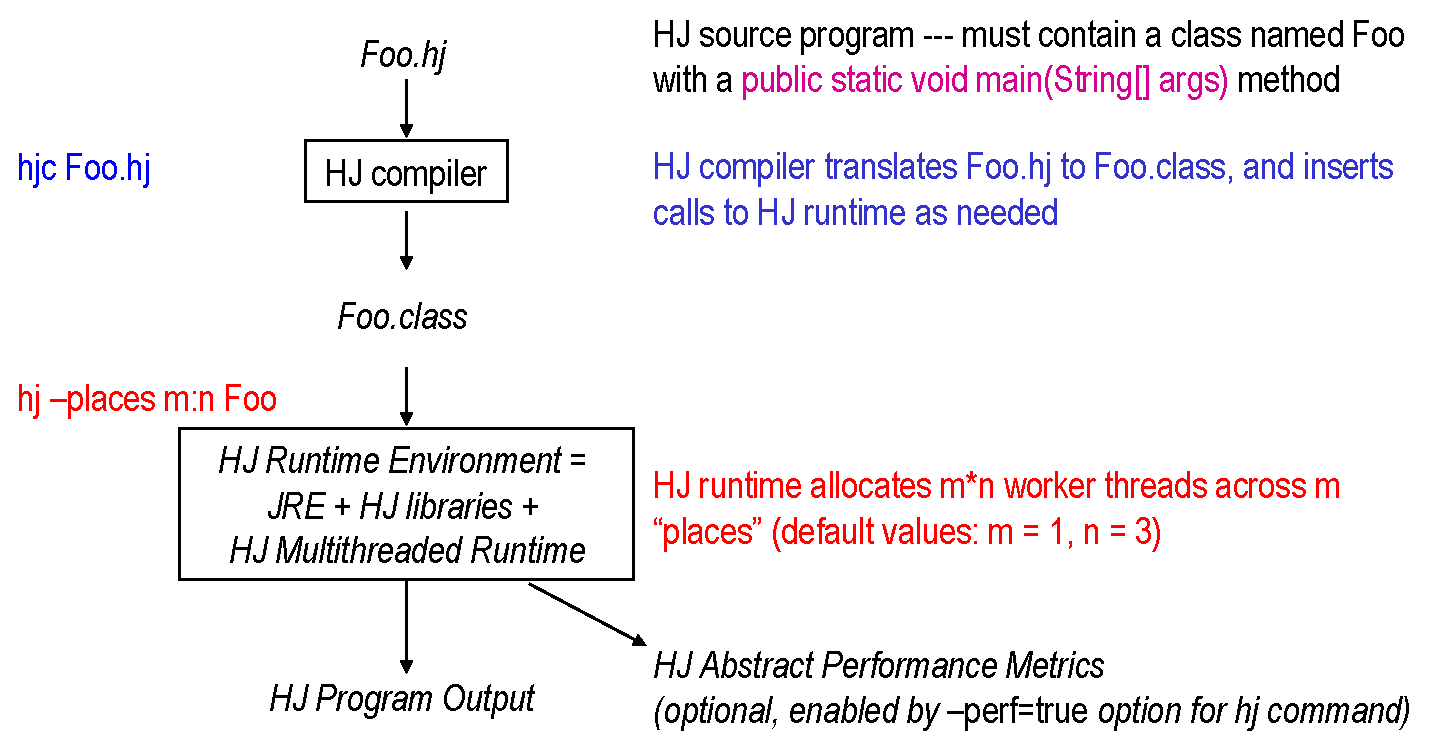
\includegraphics[width=3.25in]{../figs/hj-env}
\end{center}
\vspace{-10pt}
\caption{The HJ Compilation and Execution Environment.}
\label{fig:hj-env}
\end{figure}
\end{comment}

\begin{figure}[t]
\centering
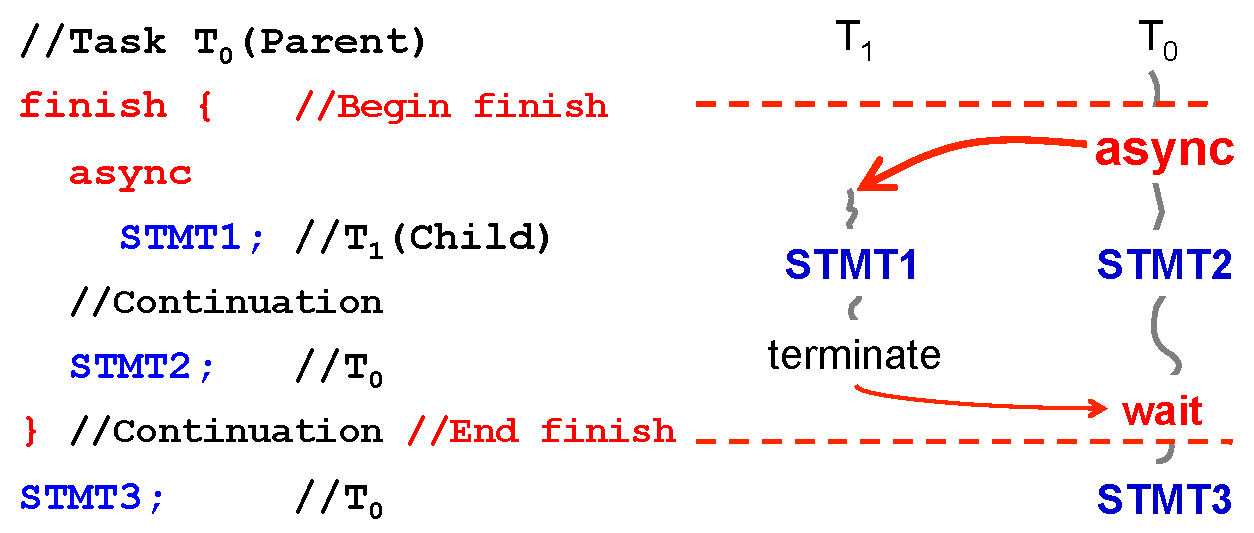
\includegraphics[width=3.25in]{../figs/async-finish}
\caption{An example with {\tt async} and {\tt finish}.}
\label{fig:async-finish}
\end{figure}

\section{Habanero Java Overview}
The overview in this paper comes from published work
describing HJ including the various figures and text
\cite{Cave:2011:HNA:2093157.2093165}. Only constructs supported in the VR system are described. The
current HJ implementation supports most of Java 5 and Java
5/6/7 libraries are accessible in HJ programs.  The HJ compiler
generates Java class files that run in a standard JVM. The HJ runtime
system provides the support for the added constructs (i.e., the system
implements, in Java, the HJ semantics).

\noindent\textbf{\texttt{async}}: \texttt{async} is a construct for
creating a new asynchronous activity.  The statement {\tt async}
$\langle${\em stmt}$\rangle$ causes the parent activity to create a
new child activity to execute {\em $\langle$stmt$\rangle$} (logically)
in parallel with the parent activity. {\em $\langle$stmt$\rangle$} can
read or write any data in the heap and can read (but not write) any
local variable belonging to the parent activity's lexical scope. The task created by \texttt{async} scheduled at the point it is declared in the
program. See \figref{fig:async-finish}.

\noindent{\bf finish: }
{\tt finish} is a generalized join operation.  The statement ``{\bf finish} $\langle${\em stmt}$\rangle$'' causes the parent
task to execute {\em $\langle$stmt$\rangle$} and then wait until all
{\tt async} tasks created within {\em $\langle$stmt$\rangle$} have completed,
including transitively spawned tasks. 
Each dynamic instance $T_A$ of an {\tt async} task has a unique {\em
  Immediately Enclosing Finish} (IEF) instance $F$ of a {\tt finish}
statement during program execution, where $F$ is the innermost {\tt
  finish} containing $T_A$~.  There is an implicit {\tt
  finish} scope surrounding the body of {\tt main()} so program
execution will only end after all {\tt async} tasks have completed.

As an example, the {\tt finish} statement in
\figref{fig:async-finish} is used by task $T_0$ to ensure that
child task $T_1$ has completed executing {\tt STMT1} before $T_0$
executes {\tt STMT3}.  If $T_1$ created a child {\tt async} task,
$T_2$ (a ``grandchild'' of $T_0$), $T_0$ will wait for both $T_1$ and
$T_2$ to complete in the {\tt finish} scope before executing {\tt
  STMT3}.

\noindent{\bf future:} 
HJ includes support for {\tt async} tasks with return
values in the form of {\tt futures}. The statement, ``{\tt final future<T> f = async<T> Expr;}''
creates a new child task to evaluate {\tt Expr} that is ready to
execute immediately.  In this case, {\tt f} contains a
``{\tt future} handle'' to the newly created task and the operation {\tt
  f.get()} can be performed to
obtain the result of the {\tt future} task.  If the {\tt future} task has not
completed as yet, the task performing the {\tt f.get()} operation
blocks until the result of {\tt Expr} becomes available.

\noindent{\bf isolated:} {\tt isolated}~$\langle${\it stmt1}$\rangle$, guarantees that each instance of $\langle${\it stmt1}$\rangle$ is performed 
in mutual exclusion with all other potentially parallel {\em interfering} instances of
{\tt isolated} statements $\langle${\it stmt2}$\rangle$.  Two instances of {\tt isolated} statements are said to interfere with each 
other if both access the same shared location, such that at least one of the accesses is a write.  

\begin{comment}
\begin{figure}
\small
\begin{verbatim} 
public static void main(String[] argv) {
   int n = Integer.parseInt(argv[0]);
   //Array Initialization to zeros
   finish {
      for (int i = 0 ; i < n ; i++) {
         async A[i] = B[i] + C[i];}}}
\end{verbatim}
\caption{An HJ program to perform vector addition.}
\label{fig:example1}
\end{figure}

\figref{fig:example1} is an HJ program to perform vector addition. The
main task creates tasks to sum each index of the vector. The finish
ensures the addition is completed before any code accesses elements of
the vector \texttt{A}.
\end{comment}
